%============================================================
%  MLP — Multilayer Perceptron
%  Aula de Graduação — Baseada em Goodfellow et al. (2016)
%============================================================
\documentclass[7pt, aspectratio=169,10pt]{beamer}

%------------------------------------------------------------
% Tema e Cores
%------------------------------------------------------------
\usetheme{Madrid}
\usecolortheme{default}
\useinnertheme{circles}

\definecolor{deepblue}{RGB}{13,71,161}
\definecolor{deepred}{RGB}{183,28,28}
\definecolor{deepgreen}{RGB}{27,94,32}
\definecolor{lightyellow}{RGB}{255,253,231}
\definecolor{lightblue}{RGB}{227,242,253}
\definecolor{lightgray}{RGB}{245,245,245}
\definecolor{accentorange}{RGB}{230,81,0}

\setbeamercolor{palette primary}{bg=deepblue,fg=white}
\setbeamercolor{palette secondary}{bg=deepblue!80,fg=white}
\setbeamercolor{palette tertiary}{bg=deepblue!60,fg=white}
\setbeamercolor{title in head/foot}{bg=deepblue,fg=white}
\setbeamercolor{author in head/foot}{bg=deepblue!80,fg=white}
\setbeamercolor{structure}{fg=deepblue}
\setbeamercolor{block title}{bg=deepblue,fg=white}
\setbeamercolor{block body}{bg=lightblue}
\setbeamercolor{block title alerted}{bg=deepred,fg=white}
\setbeamercolor{block body alerted}{bg=deepred!10}
\setbeamercolor{block title example}{bg=deepgreen,fg=white}
\setbeamercolor{block body example}{bg=deepgreen!10}

%------------------------------------------------------------
% Pacotes
%------------------------------------------------------------
\usepackage[utf8]{inputenc}
\usepackage[T1]{fontenc}
% babel removed - using UTF-8 inputenc directly
\usepackage{bm}
\usepackage{booktabs}
\usepackage{array}
\usepackage{multirow}
\usepackage{graphicx}
\usepackage{tikz}
\usetikzlibrary{shapes,arrows,positioning,calc,decorations.pathreplacing,
                matrix,fit,backgrounds,arrows.meta,chains}
\usepackage{pgfplots}
\pgfplotsset{compat=1.18}
\usepackage{listings}
\usepackage{xcolor}
\usepackage{tcolorbox}
\tcbuselibrary{skins,breakable,theorems}
\usepackage{hyperref}

%------------------------------------------------------------
% Margens e geometria do frame
%------------------------------------------------------------
\setbeamersize{text margin left=6mm, text margin right=6mm}

%------------------------------------------------------------
% Listings — Python
%------------------------------------------------------------
\lstdefinestyle{pythonstyle}{
  language=Python,
  basicstyle=\ttfamily\fontsize{7}{8}\selectfont,
  keywordstyle=\color{deepblue}\bfseries,
  stringstyle=\color{deepred},
  commentstyle=\color{deepgreen}\itshape,
  numberstyle=\tiny\color{gray},
  numbers=left, numbersep=4pt,
  frame=single, framerule=0.4pt,
  backgroundcolor=\color{lightgray},
  showstringspaces=false,
  breaklines=true,
  tabsize=4,
  xleftmargin=8pt, xrightmargin=4pt,
}
\lstset{style=pythonstyle}

%------------------------------------------------------------
% Comandos matemáticos
%------------------------------------------------------------
\newcommand{\bx}{\bm{x}}
\newcommand{\bW}{\bm{W}}
\newcommand{\bb}{\bm{b}}
\newcommand{\bz}{\bm{z}}
\newcommand{\ba}{\bm{a}}
\newcommand{\bh}{\bm{h}}
\newcommand{\by}{\bm{y}}
\newcommand{\btheta}{\bm{\theta}}
\newcommand{\R}{\mathbb{R}}
\newcommand{\E}{\mathbb{E}}
\newcommand{\sigmoid}{\sigma}
\newcommand{\pdiff}[2]{\frac{\partial #1}{\partial #2}}
\newcommand{\Loss}{\mathcal{L}}

%------------------------------------------------------------
% Título
%------------------------------------------------------------
\title[\textbf{MLP — Redes Neurais Multicamada}]
      {\textbf{Multilayer Perceptron (MLP)}\\[3pt]
       \large Fundamentos Teóricos e Implementação Prática}
\subtitle{Baseado em: \textit{Deep Learning} — Goodfellow, Bengio \& Courville (2016)}
\author[Prof.\ ---]{Disciplina: Aprendizado de Máquina Profundo}
\institute[Graduação]{\textbf{Graduação em Ciência da Computação / Engenharia}}
\date{2025}

%============================================================
\begin{document}
%============================================================

%------------------------------------------------------------
\begin{frame}
  \titlepage
\end{frame}

%------------------------------------------------------------
\begin{frame}{Agenda da Aula}
  \tableofcontents
\end{frame}

%============================================================
\section{Introdução Histórica}
%============================================================

\begin{frame}{Linha do Tempo: Das Origens às Redes Profundas}
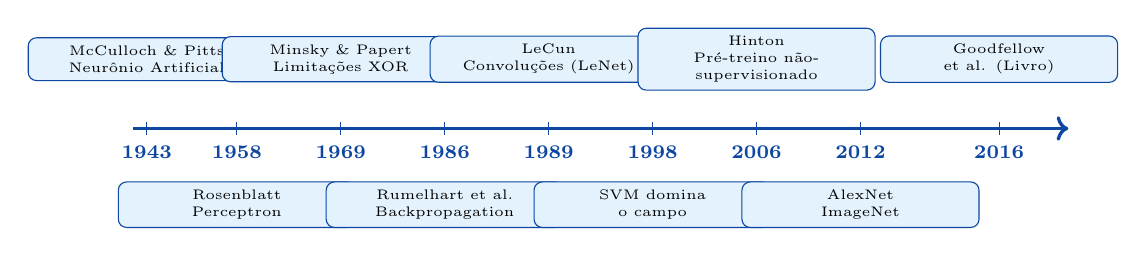
\begin{tikzpicture}[scale=0.88,
  event/.style={draw=deepblue,fill=lightblue,rounded corners=3pt,
                text width=2.8cm,align=center,font=\tiny,inner sep=3pt},
  yr/.style={font=\bfseries\scriptsize,color=deepblue}]
  % linha
  \draw[line width=1.2pt,deepblue,->] (0,0) -- (13.5,0);
  % ticks
  \foreach \x/\yr in {0.2/1943, 1.5/1958, 3.0/1969, 4.5/1986,
                       6.0/1989, 7.5/1998, 9.0/2006, 10.5/2012, 12.5/2016}{
    \draw[deepblue] (\x,0.1)--(\x,-0.1);
    \node[yr] at (\x,-0.35) {\yr};
  }
  % eventos (alternados acima/abaixo)
  \node[event] at (0.2, 1.0) {McCulloch \& Pitts\\Neurônio Artificial};
  \node[event] at (1.5,-1.1) {Rosenblatt\\Perceptron};
  \node[event] at (3.0, 1.0) {Minsky \& Papert\\Limitações XOR};
  \node[event] at (4.5,-1.1) {Rumelhart et al.\\Backpropagation};
  \node[event] at (6.0, 1.0) {LeCun\\Convoluções (LeNet)};
  \node[event] at (7.5,-1.1) {SVM domina\\o campo};
  \node[event] at (9.0, 1.0) {Hinton\\Pré-treino não-supervisionado};
  \node[event] at (10.5,-1.1) {AlexNet\\ImageNet};
  \node[event] at (12.5, 1.0) {Goodfellow\\et al. (Livro)};
\end{tikzpicture}
\vspace{2pt}
\begin{block}{}
\centering\small
O MLP é o \textbf{bloco fundamental} de todo o \textit{deep learning} moderno.
\end{block}
\end{frame}

%------------------------------------------------------------
\begin{frame}{O Neurônio Biológico e o Modelo Matemático}
\begin{columns}[T]
\column{0.45\textwidth}
\begin{block}{Neurônio Biológico}
\small
\begin{itemize}
  \item \textbf{Dendritos}: recebem sinais de entrada
  \item \textbf{Corpo celular}: integra sinais (soma ponderada)
  \item \textbf{Axônio}: transmite saída
  \item \textbf{Sinapse}: peso da conexão (plasticidade)
  \item Dispara apenas se limiar é atingido (\textit{threshold})
\end{itemize}
\end{block}
\column{0.52\textwidth}
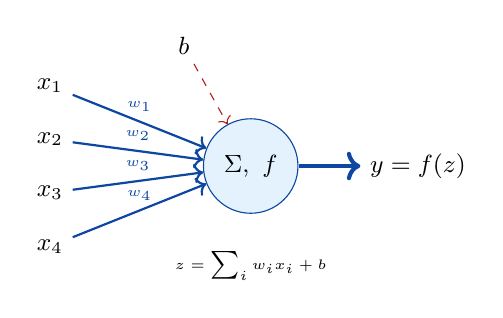
\begin{tikzpicture}[scale=0.85]
  \node[draw=deepblue,circle,fill=lightblue,minimum size=1.2cm,
        font=\small] (n) at (0,0) {$\Sigma,\ f$};
  \foreach \i/\w/\y in {1/w_1/1.2, 2/w_2/0.4, 3/w_3/-0.4, 4/w_4/-1.2}{
    \node[font=\small] (x\i) at (-3.0,\y) {$x_{\i}$};
    \draw[->,thick,deepblue] (x\i) -- node[midway,above,font=\tiny]{$\w$} (n);
  }
  \node[font=\small] (bias) at (-1.0,1.8) {$b$};
  \draw[->,dashed,deepred] (bias) -- (n);
  \node[font=\small] (out) at (2.5,0) {$y = f(z)$};
  \draw[->,thick,deepblue,line width=1.5pt] (n) -- (out);
  \node[font=\tiny,align=center] at (0,-1.5) {$z = \sum_i w_i x_i + b$};
\end{tikzpicture}
\end{columns}
\vspace{6pt}
\begin{alertblock}{Modelo McCulloch-Pitts (1943) $\to$ Perceptron (Rosenblatt, 1958)}
\small
O Perceptron introduziu \textbf{pesos ajustáveis} e uma \textbf{regra de aprendizado}; o MLP estende
isso a múltiplas camadas com funções de ativação diferenciáveis.
\end{alertblock}
\end{frame}

%============================================================
\section{Formalismo Matemático}
%============================================================

\begin{frame}{Definição Formal de um MLP}
\begin{block}{Definição (Goodfellow et al., Cap.\ 6)}
\small
Um MLP com $L$ camadas define uma função composta:
\[
  f(\bx;\,\btheta) = f^{(L)}\!\bigl(f^{(L-1)}\!\bigl(\cdots f^{(1)}(\bx)\cdots\bigr)\bigr)
\]
onde cada camada $\ell$ computa:
\[
  \boxed{\bh^{(\ell)} = f^{(\ell)}\!\bigl(\bz^{(\ell)}\bigr), \qquad
  \bz^{(\ell)} = \bW^{(\ell)}\bh^{(\ell-1)} + \bb^{(\ell)}}
\]
\end{block}
\vspace{4pt}
\begin{columns}[T]
\column{0.5\textwidth}
\begin{exampleblock}{Notação}
\small
\begin{tabular}{ll}
$\bx \in \R^{d_0}$ & vetor de entrada \\
$\bW^{(\ell)} \in \R^{d_\ell \times d_{\ell-1}}$ & matriz de pesos \\
$\bb^{(\ell)} \in \R^{d_\ell}$ & vetor de vieses \\
$\bh^{(\ell)} \in \R^{d_\ell}$ & ativação da camada $\ell$ \\
$f^{(\ell)}$ & função de ativação \\
$\btheta = \{\bW^{(\ell)},\bb^{(\ell)}\}_\ell$ & todos os parâmetros \\
\end{tabular}
\end{exampleblock}
\column{0.47\textwidth}
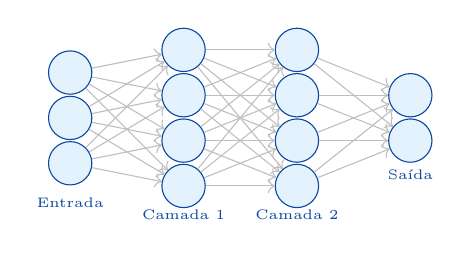
\begin{tikzpicture}[scale=0.72,
  neuron/.style={draw=deepblue,circle,fill=lightblue,minimum size=0.55cm,inner sep=1pt,font=\tiny}]
  % camadas
  % input nodes
  \node[neuron] (ia) at (0, 0.8) {};
  \node[neuron] (ib) at (0, 0.0) {};
  \node[neuron] (ic) at (0,-0.8) {};
  % hidden1 nodes
  \node[neuron] (haa) at (2, 1.2) {};
  \node[neuron] (hab) at (2, 0.4) {};
  \node[neuron] (hac) at (2,-0.4) {};
  \node[neuron] (had) at (2,-1.2) {};
  % hidden2 nodes
  \node[neuron] (hba) at (4, 1.2) {};
  \node[neuron] (hbb) at (4, 0.4) {};
  \node[neuron] (hbc) at (4,-0.4) {};
  \node[neuron] (hbd) at (4,-1.2) {};
  % output nodes
  \node[neuron] (oa) at (6, 0.4) {};
  \node[neuron] (ob) at (6,-0.4) {};
  % conexoes
  \foreach \s in {ia,ib,ic}
    \foreach \t in {haa,hab,hac,had}
      \draw[gray!50,->] (\s) -- (\t);
  \foreach \s in {haa,hab,hac,had}
    \foreach \t in {hba,hbb,hbc,hbd}
      \draw[gray!50,->] (\s) -- (\t);
  \foreach \s in {hba,hbb,hbc,hbd}
    \foreach \t in {oa,ob}
      \draw[gray!50,->] (\s) -- (\t);
  % rotulos
  \node[font=\tiny,deepblue] at (0,-1.5) {Entrada};
  \node[font=\tiny,deepblue] at (2,-1.7) {Camada 1};
  \node[font=\tiny,deepblue] at (4,-1.7) {Camada 2};
  \node[font=\tiny,deepblue] at (6,-1.0) {Sa\'ida};
\end{tikzpicture}
\end{columns}
\end{frame}

%------------------------------------------------------------
\begin{frame}{Cálculo Manual — Rede Pequena (Exemplo Detalhado)}
\begin{block}{Configuração: 2 entradas $\to$ 2 neurônios ocultos $\to$ 1 saída}
\small
Ativação oculta: ReLU$(\cdot)$; saída: sigmoide $\sigma(\cdot)$.
\end{block}
\begin{columns}[T]
\column{0.52\textwidth}
\textbf{Parâmetros dados:}
\[
\bW^{(1)}=\begin{pmatrix}1 & 2\\ -1 & 1\end{pmatrix},\quad
\bb^{(1)}=\begin{pmatrix}0\\1\end{pmatrix}
\]
\[
\bW^{(2)}=\begin{pmatrix}3 & -2\end{pmatrix},\quad
\bb^{(2)}=\begin{pmatrix}-1\end{pmatrix}
\]
\textbf{Entrada:} $\bx=(1,\,-1)^\top$

\vspace{6pt}
\textbf{Passo 1 — pré-ativação camada 1:}
\[
\bz^{(1)} = \bW^{(1)}\bx + \bb^{(1)}
= \begin{pmatrix}1(1)+2(-1)\\-1(1)+1(-1)\end{pmatrix}+\begin{pmatrix}0\\1\end{pmatrix}
= \begin{pmatrix}-1\\-1\end{pmatrix}
\]

\column{0.45\textwidth}
\textbf{Passo 2 — ativação ReLU:}
\[
\bh^{(1)} = \max(\bz^{(1)}, \bm{0}) = \begin{pmatrix}0\\0\end{pmatrix}
\]

\textbf{Passo 3 — pré-ativação saída:}
\[
z^{(2)} = \bW^{(2)}\bh^{(1)} + b^{(2)}
= 3(0)+(-2)(0)+(-1) = -1
\]

\textbf{Passo 4 — ativação sigmoide:}
\[
\hat{y} = \sigma(-1) = \frac{1}{1+e^{1}} \approx \boxed{0.269}
\]

\begin{alertblock}{Interpretação}
\tiny
A entrada $(1,-1)$ resulta em probabilidade $\approx 26.9\%$ para a classe positiva.
\end{alertblock}
\end{columns}
\end{frame}

%============================================================
\section{Funções de Ativação}
%============================================================

\begin{frame}{Por que Funções de Ativação São Necessárias?}
\begin{alertblock}{Teorema: Composição de Funções Lineares é Linear}
\small
Se $f^{(\ell)}(\bz) = \bz$ (identidade), então:
\[
f(\bx) = \bW^{(L)}\!\bigl(\bW^{(L-1)}\!\bigl(\cdots\bW^{(1)}\bx+\bb^{(1)}\cdots\bigr)\bigr)
= \underbrace{\bW_{\text{eq}}}_{\text{único }W}\bx + \bb_{\text{eq}}
\]
\textbf{Uma rede profunda linear é equivalente a uma rede de camada única!}
A profundidade não acrescenta poder expressivo.
\end{alertblock}
\vspace{6pt}
\begin{columns}[T]
\column{0.48\textwidth}
\begin{block}{Requisitos de uma Boa Ativação}
\small
\begin{itemize}
  \item \textbf{Não-linearidade}: poder de aproximação universal
  \item \textbf{Diferenciabilidade}: viabiliza backprop
  \item \textbf{Gradientes estáveis}: evita vanishing/exploding
  \item \textbf{Eficiência computacional}
\end{itemize}
\end{block}
\column{0.48\textwidth}
\begin{block}{Teorema de Aproximação Universal}
\small
Um MLP com \textbf{uma camada oculta} e ativação não-linear pode aproximar qualquer função contínua em um compacto de $\R^n$ com precisão arbitrária (Hornik, 1991).
\\\textit{Mas: pode precisar de exponencialmente muitos neurônios.}
\end{block}
\end{columns}
\end{frame}

%------------------------------------------------------------
\begin{frame}{Funções de Ativação Clássicas}
\begin{columns}[T]
\column{0.48\textwidth}

\begin{block}{Sigmoide $\sigma(z) = \frac{1}{1+e^{-z}}$}
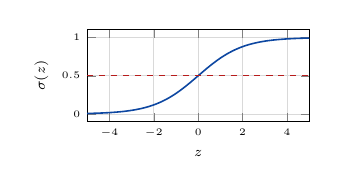
\begin{tikzpicture}[scale=0.72]
\begin{axis}[xlabel={$z$},ylabel={$\sigma(z)$},
  width=5.5cm,height=3.2cm,
  xmin=-5,xmax=5,ymin=-0.1,ymax=1.1,
  grid=major,grid style={gray!30},
  tick label style={font=\tiny},
  label style={font=\scriptsize}]
\addplot[deepblue,thick,domain=-5:5,samples=100] {1/(1+exp(-x))};
\addplot[deepred,dashed,domain=-5:5] {0.5};
\end{axis}
\end{tikzpicture}
\\\small $\sigma'(z)=\sigma(z)(1-\sigma(z)) \leq 0.25$
\\\textbf{Problema:} saturação $\Rightarrow$ \textit{vanishing gradient}
\end{block}

\begin{block}{Tangente Hiperbólica $\tanh(z)$}
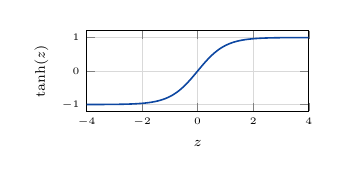
\begin{tikzpicture}[scale=0.72]
\begin{axis}[xlabel={$z$},ylabel={$\tanh(z)$},
  width=5.5cm,height=3.0cm,
  xmin=-4,xmax=4,ymin=-1.2,ymax=1.2,
  grid=major,grid style={gray!30},
  tick label style={font=\tiny},
  label style={font=\scriptsize}]
\addplot[deepblue,thick,domain=-4:4,samples=100] {tanh(x)};
\end{axis}
\end{tikzpicture}
\\\small $\tanh(z) = 2\sigma(2z)-1$, centrada em zero.
\\\textbf{Melhor} que sigmoid, mas ainda satura.
\end{block}

\column{0.48\textwidth}

\begin{block}{ReLU $f(z)=\max(0,z)$ (Nair \& Hinton, 2010)}
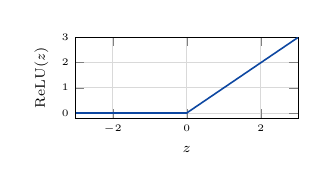
\begin{tikzpicture}[scale=0.72]
\begin{axis}[xlabel={$z$},ylabel={ReLU$(z)$},
  width=5.5cm,height=3.0cm,
  xmin=-3,xmax=3,ymin=-0.2,ymax=3,
  grid=major,grid style={gray!30},
  tick label style={font=\tiny},
  label style={font=\scriptsize}]
\addplot[deepblue,thick,domain=-3:0] {0};
\addplot[deepblue,thick,domain=0:3] {x};
\end{axis}
\end{tikzpicture}
\\\small $f'(z) = \mathbf{1}[z>0]$ — gradiente constante para $z>0$!
\\\textbf{Problema}: neurônios mortos (\textit{dying ReLU})
\end{block}

\begin{block}{Variantes Modernas}
\small
\begin{tabular}{ll}
\textbf{Leaky ReLU} & $\max(\alpha z, z),\ \alpha\!\approx\!0.01$ \\
\textbf{ELU} & $z$ se $z>0$; $\alpha(e^z-1)$ caso contrário \\
\textbf{GELU} & $z\,\Phi(z)$ (usado em Transformers) \\
\textbf{Swish} & $z\,\sigma(\beta z)$ (Google, 2017) \\
\end{tabular}
\end{block}

\end{columns}
\end{frame}

%------------------------------------------------------------
\begin{frame}{Softmax — Ativação para Classificação Multiclasse}
\begin{block}{Definição}
\[
  \text{softmax}(\bz)_k = \frac{e^{z_k}}{\sum_{j=1}^{K} e^{z_j}}, \qquad k=1,\ldots,K
\]
\end{block}
\begin{columns}[T]
\column{0.48\textwidth}
\begin{exampleblock}{Propriedades}
\small
\begin{itemize}
  \item Saída $\in (0,1)$ e $\sum_k \text{softmax}(\bz)_k = 1$
  \item Interpreta-se como \textbf{distribuição de probabilidade}
  \item Softmax é monotônica: preserva ordenação de $\bz$
  \item Combinada com \textbf{cross-entropy}: gradientes limpos
\end{itemize}
\end{exampleblock}
\begin{alertblock}{Estabilidade Numérica}
\small
Na prática, use:
$\text{softmax}(\bz)_k = \dfrac{e^{z_k - \max_j z_j}}{\sum_j e^{z_j-\max_j z_j}}$
\end{alertblock}
\column{0.48\textwidth}
\begin{exampleblock}{Exemplo Numérico}
\small
$\bz = (2.0,\ 1.0,\ 0.1)$
\begin{align*}
e^{2.0} &= 7.389,\quad e^{1.0}=2.718,\quad e^{0.1}=1.105\\
S &= 11.212\\
\text{softmax} &= (0.659,\; 0.242,\; 0.099)
\end{align*}
Classe 1 tem probabilidade $\approx 65.9\%$.
\end{exampleblock}
\end{columns}
\end{frame}

%============================================================
\section{O Problema XOR e a Necessidade de Não-Linearidade}
%============================================================

\begin{frame}{XOR: Por que o Perceptron Simples Falha}
\begin{columns}[T]
\column{0.45\textwidth}
\begin{block}{Tabela-Verdade XOR}
\centering\small
\begin{tabular}{cccc}
\toprule
$x_1$ & $x_2$ & XOR & Classe \\
\midrule
0 & 0 & 0 & $-$ \\
0 & 1 & 1 & $+$ \\
1 & 0 & 1 & $+$ \\
1 & 1 & 0 & $-$ \\
\bottomrule
\end{tabular}
\end{block}
\vspace{8pt}
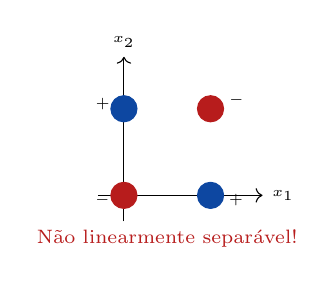
\begin{tikzpicture}[scale=1.1]
  \draw[->] (-0.3,0)--(1.6,0) node[right,font=\tiny]{$x_1$};
  \draw[->] (0,-0.3)--(0,1.6) node[above,font=\tiny]{$x_2$};
  \node[draw=deepred,fill=deepred,circle,minimum size=6pt] at (0,0) {};
  \node[draw=deepblue,fill=deepblue,circle,minimum size=6pt] at (0,1) {};
  \node[draw=deepblue,fill=deepblue,circle,minimum size=6pt] at (1,0) {};
  \node[draw=deepred,fill=deepred,circle,minimum size=6pt] at (1,1) {};
  \node[font=\tiny,right] at (1.1,1.1) {$-$};
  \node[font=\tiny,right] at (1.1,-0.05) {$+$};
  \node[font=\tiny,left] at (-0.05,1.05) {$+$};
  \node[font=\tiny,left] at (-0.05,-0.05) {$-$};
  \node[font=\scriptsize,deepred] at (0.5,-0.5) {Não linearmente separável!};
\end{tikzpicture}
\column{0.52\textwidth}
\begin{alertblock}{Prova Formal de Impossibilidade}
\small
Um perceptron linear busca $w_1,w_2,b$ tal que:
\begin{align*}
  w_1(0)+w_2(0)+b &\leq 0 \quad (0,0)\to- \\
  w_1(0)+w_2(1)+b &> 0 \quad (0,1)\to+ \\
  w_1(1)+w_2(0)+b &> 0 \quad (1,0)\to+ \\
  w_1(1)+w_2(1)+b &\leq 0 \quad (1,1)\to-
\end{align*}
Somando linhas 1 e 4: $w_1+w_2+2b \leq 0$\\
Somando linhas 2 e 3: $w_1+w_2+2b > 0$\\
\textbf{Contradição} $\Rightarrow$ impossível!
\end{alertblock}
\begin{block}{Conclusão (Minsky \& Papert, 1969)}
\small
Perceptrons de camada única são fundamentalmente limitados para problemas não-linearmente separáveis. $\Rightarrow$ Precisamos de \textbf{camadas ocultas}.
\end{block}
\end{columns}
\end{frame}

%------------------------------------------------------------
\begin{frame}{XOR Resolvido por MLP — Via Equações Normais}
\begin{block}{Arquitetura: $2 \to 2 \to 1$ com ReLU oculta, sigmoide na saída}
\end{block}
\begin{columns}[T]
\column{0.50\textwidth}
\small
\textbf{Solução clássica (Goodfellow et al., Eq.\ 6.1):}
\[
\bW^{(1)}=\begin{pmatrix}1&1\\1&1\end{pmatrix},\;
\bb^{(1)}=\begin{pmatrix}0\\-1\end{pmatrix}
\]
\[
\bW^{(2)}=\begin{pmatrix}1&-2\end{pmatrix},\;
\bb^{(2)}=0
\]
\textbf{Para $\bx=(0,1)$:}
\[
\bz^{(1)}=\begin{pmatrix}1\\0\end{pmatrix},\;
\bh^{(1)}=\text{ReLU}\!\begin{pmatrix}1\\0\end{pmatrix}=\begin{pmatrix}1\\0\end{pmatrix}
\]
\[
z^{(2)} = 1(1)+(-2)(0)+0 = 1 \Rightarrow \hat{y}=1\ (\checkmark)
\]
\column{0.47\textwidth}
\small
\textbf{Tabela completa:}
\begin{center}
\begin{tabular}{cc|cc|c|c}
\toprule
$x_1$ & $x_2$ & $h_1^{(1)}$ & $h_2^{(1)}$ & $z^{(2)}$ & XOR\\
\midrule
0 & 0 & 0 & 0 & 0 & 0 \\
0 & 1 & 1 & 0 & 1 & 1 \\
1 & 0 & 1 & 0 & 1 & 1 \\
1 & 1 & 2 & 1 & 0 & 0 \\
\bottomrule
\end{tabular}
\end{center}
\begin{exampleblock}{Insight Fundamental}
\small
A camada oculta \textbf{recodifica o espaço de entrada} criando uma representação linearmente separável. Esta é a essência do aprendizado de representações!
\end{exampleblock}
\end{columns}
\end{frame}

%============================================================
\section{Design de Arquiteturas}
%============================================================

\begin{frame}{Princípios de Design de Arquiteturas}
\begin{columns}[T]
\column{0.48\textwidth}
\begin{block}{Hiperparâmetros Estruturais}
\small
\begin{itemize}
  \item \textbf{Profundidade} $L$: número de camadas
  \item \textbf{Largura} $d_\ell$: neurônios por camada
  \item \textbf{Tipo de ativação} por camada
  \item \textbf{Conectividade}: densa, esparsa, convolucional
  \item \textbf{Skip connections} (ResNets)
\end{itemize}
\end{block}
\begin{block}{Profundidade vs.\ Largura}
\small
\begin{itemize}
  \item Redes mais \textbf{profundas} $\Rightarrow$ hierarquia de features
  \item Redes mais \textbf{largas} $\Rightarrow$ memorização bruta
  \item Empiricamente: profundidade $>$ largura para generalização
  \item Teoricamente: funções exponencialmente mais expressivas com camadas (Montufar et al., 2014)
\end{itemize}
\end{block}
\column{0.48\textwidth}
\begin{block}{Regras Práticas}
\small
\begin{tabular}{lp{3.4cm}}
\textbf{Saída regressão} & $1$ neurônio linear \\
\textbf{Classificação bin.} & $1$ neurônio + sigmoid \\
\textbf{Classif.\ multi} & $K$ neurônios + softmax \\
\textbf{Largura oculta} & $64 \to 256 \to 1024$ (decrescente) \\
\textbf{Profundidade} & $2$--$5$ para tabular; mais para imagem \\
\end{tabular}
\end{block}
\begin{alertblock}{Aviso: Não há Teoria Completa}
\small
O design de arquitetura é amplamente empírico. Técnicas como NAS (\textit{Neural Architecture Search}) automatizam parte da busca.
\end{alertblock}
\end{columns}
\end{frame}

%============================================================
\section{Funções de Perda}
%============================================================

\begin{frame}{Teoria das Funções de Perda — Motivação}
\begin{block}{Princípio de Máxima Verossimilhança (MLE)}
\small
Dado um dataset $\mathcal{D}=\{(\bx^{(i)},y^{(i)})\}_{i=1}^N$, buscamos:
\[
\btheta^* = \arg\max_{\btheta} \log p(\mathcal{D};\btheta)
= \arg\max_{\btheta} \sum_{i=1}^N \log p(y^{(i)}|\bx^{(i)};\btheta)
\]
\[
\equiv \arg\min_{\btheta} -\frac{1}{N}\sum_{i=1}^N \log p(y^{(i)}|\bx^{(i)};\btheta) = \mathcal{L}(\btheta)
\]
\end{block}
\vspace{4pt}
\begin{exampleblock}{Conexão com Entropia Cruzada}
\small
Maximizar log-verossimilhança é equivalente a minimizar a \textbf{divergência KL} entre a distribuição empírica dos dados e a distribuição do modelo:
\[
D_{KL}(p_{\text{dados}}\,\|\,p_{\text{modelo}}) = -\E_{p_{\text{dados}}}[\log p_{\text{modelo}}] + \text{const}
\]
A função de perda emerge naturalmente da escolha do modelo probabilístico!
\end{exampleblock}
\end{frame}

%------------------------------------------------------------
\begin{frame}{Perdas para Regressão}
\begin{columns}[T]
\column{0.48\textwidth}
\begin{block}{Mean Squared Error (MSE) — $\ell_2$}
\[
\mathcal{L}_{\text{MSE}} = \frac{1}{N}\sum_{i=1}^N \bigl(y^{(i)}-\hat{y}^{(i)}\bigr)^2
\]
\small
\begin{itemize}
  \item Assume $p(y|\bx) = \mathcal{N}(\hat{y},\sigma^2)$ (ruído Gaussiano)
  \item Penaliza erros grandes \textbf{quadraticamente}
  \item \textbf{Sensível a outliers} (quadrado amplifica)
  \item Gradiente suave e convexo
  \item Mais usado na prática para regressão
\end{itemize}
\end{block}
\begin{block}{Mean Absolute Error (MAE) — $\ell_1$}
\[
\mathcal{L}_{\text{MAE}} = \frac{1}{N}\sum_{i=1}^N \bigl|y^{(i)}-\hat{y}^{(i)}\bigr|
\]
\small
\begin{itemize}
  \item Assume $p(y|\bx) \propto e^{-|y-\hat{y}|/\lambda}$ (Laplace)
  \item \textbf{Robusto a outliers}
  \item Gradiente descontinuo em $0$: use Huber na prática
\end{itemize}
\end{block}
\column{0.48\textwidth}
\begin{block}{Huber Loss (Combinação)}
\[
\mathcal{L}_\delta = \begin{cases} \tfrac{1}{2}r^2 & |r|\leq\delta \\ \delta(|r|-\tfrac{\delta}{2}) & |r|>\delta \end{cases}
\]
\small $r = y-\hat{y}$. Quadrática perto de zero, linear para outliers.
\end{block}
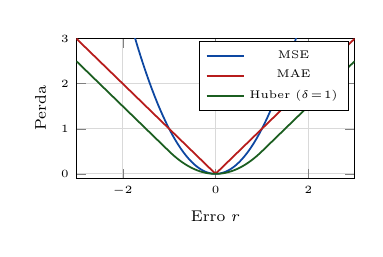
\begin{tikzpicture}[scale=0.80]
\begin{axis}[xlabel={Erro $r$},ylabel={Perda},
  width=6cm,height=3.8cm,
  xmin=-3,xmax=3,ymin=-0.1,ymax=3,
  grid=major,grid style={gray!30},
  tick label style={font=\tiny},
  label style={font=\scriptsize},
  legend style={font=\tiny,at={(0.98,0.98)},anchor=north east}]
\addplot[deepblue,thick,domain=-3:3,samples=100] {x*x};
\addlegendentry{MSE}
\addplot[deepred,thick,domain=-3:3,samples=100] {abs(x)};
\addlegendentry{MAE}
\addplot[deepgreen,thick,domain=-3:3,samples=100] 
  {(abs(x)<=1)*0.5*x*x + (abs(x)>1)*(abs(x)-0.5)};
\addlegendentry{Huber ($\delta\!=\!1$)}
\end{axis}
\end{tikzpicture}
\end{columns}
\end{frame}

%------------------------------------------------------------
\begin{frame}{Perdas para Classificação}
\begin{columns}[T]
\column{0.48\textwidth}
\begin{block}{Binary Cross-Entropy (BCE)}
\[
\mathcal{L}_{\text{BCE}} = -\frac{1}{N}\sum_i \bigl[y_i\log\hat{y}_i + (1-y_i)\log(1-\hat{y}_i)\bigr]
\]
\begin{itemize}
  \item Para classificação binária com saída sigmoid
  \item Deriva de $p(y|\bx) = \text{Bernoulli}(\hat{y})$
  \item Gradiente: $\hat{y} - y$ (elegante com sigmoid!)
\end{itemize}
\end{block}
\column{0.48\textwidth}
\begin{block}{Categorical Cross-Entropy (CCE)}
\[
\mathcal{L}_{\text{CCE}} = -\frac{1}{N}\sum_i \sum_{k=1}^K y_{i,k}\log\hat{y}_{i,k}
\]
\begin{itemize}
  \item Para $K$ classes com saída softmax
  \item Com \textit{one-hot}: $\mathcal{L} = -\frac{1}{N}\sum_i \log\hat{y}_{i,c_i}$
\end{itemize}
\end{block}
\end{columns}
\begin{alertblock}{Regra Geral}
\small
\begin{tabular}{ll}
Regressão & MSE ou Huber \\
Classif.\ binária & BCE + sigmoid \\
Classif.\ multi & CCE + softmax \\
\end{tabular}
\end{alertblock}
\end{frame}

%============================================================
\section{Backpropagation e Grafos Computacionais}
%============================================================

\begin{frame}{Histórico do Backpropagation}
\begin{columns}[T]
\column{0.55\textwidth}
\begin{block}{Linha do Tempo}
\small
\begin{itemize}
  \item \textbf{1960}: Kelley e Bryson — princípio da cadeia em controle ótimo
  \item \textbf{1970}: Linnainmaa — diferenciação automática reversa
  \item \textbf{1974}: Werbos — aplica em redes neurais (dissertação)
  \item \textbf{1986}: \textbf{Rumelhart, Hinton \& Williams} — populariza em redes neurais
  \item \textbf{1988}: LeCun aplica em reconhecimento de dígitos
  \item \textbf{2000s}: Frameworks de diferenciação automática (Theano)
  \item \textbf{2015}: TensorFlow, PyTorch — autograd automático
\end{itemize}
\end{block}
\column{0.42\textwidth}
\begin{alertblock}{O que é Backprop?}
\small
\textbf{Não} é um algoritmo de otimização — é um método eficiente para calcular gradientes usando a \textbf{regra da cadeia} de forma reversa (``backward pass'').
\end{alertblock}
\begin{block}{Complexidade}
\small
\begin{itemize}
  \item \textit{Forward pass}: $O(|\btheta|)$
  \item \textit{Backward pass}: $O(|\btheta|)$ 
  \item Custo total: constante $\times$ forward!
\end{itemize}
\end{block}
\end{columns}
\end{frame}

%------------------------------------------------------------
\begin{frame}{Grafos Computacionais}
\begin{columns}[T]
\column{0.48\textwidth}
\begin{block}{Definição}
\small
Um \textbf{grafo computacional} é um DAG (Grafo Acíclico Dirigido) onde:
\begin{itemize}
  \item \textbf{Nós}: variáveis (escalares, vetores, tensores)
  \item \textbf{Arestas}: operações computacionais
  \item A topologia determina a ordem de avaliação e dos gradientes
\end{itemize}
\end{block}
\begin{exampleblock}{Exemplo: $z = (x+y)\cdot w$}
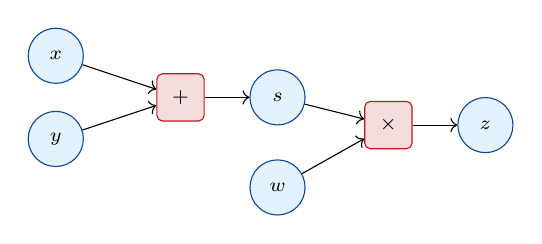
\begin{tikzpicture}[scale=0.88,
  node/.style={draw=deepblue,circle,fill=lightblue,font=\scriptsize,minimum size=0.7cm},
  op/.style={draw=deepred,rectangle,fill=deepred!15,font=\scriptsize,rounded corners=2pt,minimum size=0.6cm}]
  \node[node] (x) at (0,1.0) {$x$};
  \node[node] (y) at (0,-0.2) {$y$};
  \node[op] (add) at (1.8,0.4) {$+$};
  \node[node] (s) at (3.2,0.4) {$s$};
  \node[node] (w) at (3.2,-0.9) {$w$};
  \node[op] (mul) at (4.8,0.0) {$\times$};
  \node[node] (z) at (6.2,0.0) {$z$};
  \draw[->] (x)--(add); \draw[->] (y)--(add);
  \draw[->] (add)--(s); \draw[->] (s)--(mul);
  \draw[->] (w)--(mul); \draw[->] (mul)--(z);
\end{tikzpicture}
\end{exampleblock}
\column{0.48\textwidth}
\begin{block}{Diferenciação em Grafos}
\small
Para calcular $\pdiff{\mathcal{L}}{x}$, percorremos o grafo de trás para frente:
\[
\pdiff{\mathcal{L}}{x} = \pdiff{\mathcal{L}}{z}\cdot\pdiff{z}{s}\cdot\pdiff{s}{x}
= \pdiff{\mathcal{L}}{z}\cdot w \cdot 1
\]
\end{block}
\begin{alertblock}{PyTorch vs TensorFlow}
\small
\textbf{PyTorch}: grafo \textit{dinâmico} (define-by-run)\\
\textbf{TensorFlow 1.x}: grafo \textit{estático} (define-then-run)\\
\textbf{TF 2.x / JAX}: ambos modos disponíveis
\end{alertblock}
\begin{block}{}
\small
\texttt{tensor.backward()} em PyTorch percorre automaticamente o grafo e acumula gradientes em \texttt{.grad}.
\end{block}
\end{columns}
\end{frame}

%------------------------------------------------------------
\begin{frame}{Backpropagation — Matemática Completa}
\begin{block}{Regra da Cadeia Vetorial (Jacobiana)}
\small
Para $\bz = f(\bx)$ e $\mathcal{L}$ escalar:
\[
\pdiff{\mathcal{L}}{\bx} = \left(\pdiff{\bz}{\bx}\right)^\top \pdiff{\mathcal{L}}{\bz}
\]
onde $\pdiff{\bz}{\bx} \in \R^{m\times n}$ é a matriz Jacobiana.
\end{block}
\begin{columns}[T]
\column{0.50\textwidth}
\small\textbf{Gradientes por camada:}

Para a camada $\ell$: $\bz^{(\ell)} = \bW^{(\ell)}\bh^{(\ell-1)}+\bb^{(\ell)}$, $\bh^{(\ell)} = f(\bz^{(\ell)})$

\vspace{4pt}
\textbf{Definimos} $\bm{\delta}^{(\ell)} \equiv \pdiff{\mathcal{L}}{\bz^{(\ell)}}$ (\textit{sinal de erro})
\[
\bm{\delta}^{(L)} = \pdiff{\mathcal{L}}{\bz^{(L)}} \quad \text{(depende da perda)}
\]
\[
\bm{\delta}^{(\ell)} = \left(\bW^{(\ell+1)}\right)^\top \bm{\delta}^{(\ell+1)} \odot f'\!\left(\bz^{(\ell)}\right)
\]
\[
\pdiff{\mathcal{L}}{\bW^{(\ell)}} = \bm{\delta}^{(\ell)}\left(\bh^{(\ell-1)}\right)^\top
\]
\[
\pdiff{\mathcal{L}}{\bb^{(\ell)}} = \bm{\delta}^{(\ell)}
\]
\column{0.47\textwidth}
\begin{exampleblock}{Interpretação de $\odot$}
\small
$\odot$ denota produto elemento a elemento (Hadamard). A multiplicação por $f'(\bz^{(\ell)})$ é a \textbf{gate} do gradiente.
\end{exampleblock}
\begin{alertblock}{Vanishing Gradient}
\small
Se $\max |f'| < 1$ (sigmoid: $\leq 0.25$), então $\|\bm{\delta}^{(\ell)}\|$ decresce exponencialmente com a profundidade $L-\ell$.
$\Rightarrow$ \textbf{ReLU} resolve em grande parte este problema.
\end{alertblock}
\end{columns}
\end{frame}

%------------------------------------------------------------
\begin{frame}{Backprop — Exemplo Numérico Completo}
\small
\textbf{Rede:} $x\to h=\text{ReLU}(wx+b)\to\hat{y}=h \cdot v \to \mathcal{L}=\tfrac{1}{2}(\hat{y}-y)^2$

\textbf{Valores:} $x=2$, $w=1$, $b=-1$, $v=3$, $y=5$.
\begin{columns}[T]
\column{0.48\textwidth}
\textbf{Forward pass:}
\begin{align*}
  z &= wx+b = 1(2)+(-1) = 1\\
  h &= \text{ReLU}(1) = 1\\
  \hat{y} &= vh = 3(1) = 3\\
  \mathcal{L} &= \tfrac{1}{2}(3-5)^2 = 2
\end{align*}
\column{0.48\textwidth}
\textbf{Backward pass:}
\begin{align*}
  \pdiff{\mathcal{L}}{\hat{y}} &= \hat{y}-y = 3-5 = -2\\
  \pdiff{\mathcal{L}}{v} &= \pdiff{\mathcal{L}}{\hat{y}}\cdot h = (-2)(1)=-2\\
  \pdiff{\mathcal{L}}{h} &= \pdiff{\mathcal{L}}{\hat{y}}\cdot v = (-2)(3)=-6\\
  \pdiff{\mathcal{L}}{z} &= \pdiff{\mathcal{L}}{h}\cdot\mathbf{1}[z>0]=(-6)(1)=-6\\
  \pdiff{\mathcal{L}}{w} &= \pdiff{\mathcal{L}}{z}\cdot x = (-6)(2) = -12\\
  \pdiff{\mathcal{L}}{b} &= \pdiff{\mathcal{L}}{z}\cdot 1 = -6
\end{align*}
\end{columns}
\begin{exampleblock}{Atualização (SGD com $\eta=0.1$)}
$w \leftarrow 1 - 0.1(-12) = 2.2$,\quad
$b \leftarrow -1 - 0.1(-6) = -0.4$,\quad
$v \leftarrow 3 - 0.1(-2) = 3.2$
\end{exampleblock}
\end{frame}

%============================================================
\section{Regularização}
%============================================================

\begin{frame}{Penalidades de Norma de Parâmetros}
\begin{block}{Regularização $\ell_2$ (Weight Decay)}
\[
\tilde{\mathcal{L}}(\btheta) = \mathcal{L}(\btheta) + \frac{\lambda}{2}\|\btheta\|_2^2
\]
\small
\begin{itemize}
  \item Assume prior $\btheta \sim \mathcal{N}(0, \lambda^{-1}\mathbf{I})$ (MAP)
  \item Penaliza pesos grandes igualmente
  \item Gradiente extra: $\lambda\btheta$
  \item Efeito: encolhe pesos em direção a zero (\textit{shrinkage})
  \item SGD com $\ell_2$: ``\textit{weight decay}''
\end{itemize}
\end{block}
\end{frame}

\begin{frame}
  \begin{block}{Regularização $\ell_1$ (Lasso)}
\[
\tilde{\mathcal{L}}(\btheta) = \mathcal{L}(\btheta) + \lambda\|\btheta\|_1
\]
\small
\begin{itemize}
  \item Assume prior Laplace
  \item Promove \textbf{esparsidade} (muitos pesos $=0$)
  \item Menos usado em deep learning
\end{itemize}
\end{block}
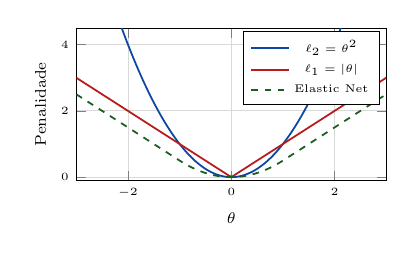
\begin{tikzpicture}[scale=0.80]
\begin{axis}[xlabel={$\theta$},ylabel={Penalidade},
  width=6.5cm,height=4.0cm,
  xmin=-3,xmax=3,ymin=-0.1,ymax=4.5,
  grid=major,grid style={gray!30},
  tick label style={font=\tiny},
  label style={font=\scriptsize},
  legend style={font=\tiny,at={(0.98,0.98)},anchor=north east}]
\addplot[deepblue,thick,domain=-3:3,samples=100] {x*x};
\addlegendentry{$\ell_2 = \theta^2$}
\addplot[deepred,thick,domain=-3:3,samples=100] {abs(x)};
\addlegendentry{$\ell_1 = |\theta|$}
\addplot[deepgreen,thick,dashed,domain=-3:3,samples=100] 
  {(abs(x)<=1)*0.5*x*x + (abs(x)>1)*(abs(x)-0.5)};
\addlegendentry{Elastic Net}
\end{axis}
\end{tikzpicture}
\begin{alertblock}{Elastic Net}
\small
Combinação: $\lambda_1\|\btheta\|_1 + \lambda_2\|\btheta\|_2^2$. Tem benefícios de ambas as penalidades.
\end{alertblock}

\end{frame}

%------------------------------------------------------------
\begin{frame}{Dropout}
\begin{columns}[T]
\column{0.52\textwidth}
\begin{block}{Definição (Srivastava et al., 2014)}
\small
Durante o treino, cada neurônio (exceto saída) é zerado com probabilidade $p$ (tipicamente $0.5$):
\[
\tilde{h}_j = \frac{r_j \cdot h_j}{1-p}, \quad r_j \sim \text{Bernoulli}(1-p)
\]
O fator $1/(1-p)$ (\textit{inverted dropout}) garante que $\E[\tilde{h}_j] = h_j$.
\end{block}
\begin{exampleblock}{Na Inferência}
\small
Dropout é desligado. Use todos os neurônios com pesos completos. O ensemble implícito é ``integrado'' automaticamente.
\end{exampleblock}
\column{0.45\textwidth}
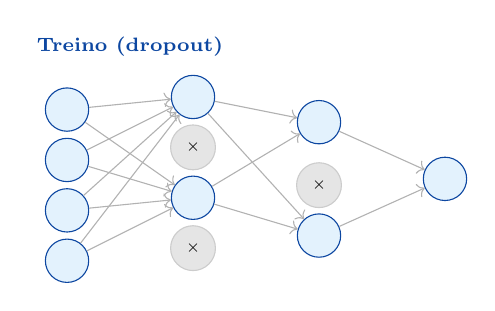
\begin{tikzpicture}[scale=0.80,
  n/.style={draw=deepblue,circle,fill=lightblue,minimum size=0.55cm,font=\tiny},
  nd/.style={draw=gray!40,circle,fill=gray!20,minimum size=0.55cm,font=\tiny}]
  \node[font=\scriptsize,deepblue] at (1.0,2.8) {\textbf{Treino (dropout)}};
  % input layer
  \node[n] (ina) at (0, 1.8) {};
  \node[n] (inb) at (0, 1.0) {};
  \node[n] (inc) at (0, 0.2) {};
  \node[n] (ind) at (0,-0.6) {};
  % hidden 1 - alguns dropados
  \node[n]  (h1a) at (2, 2.0) {};
  \node[nd] (h1b) at (2, 1.2) {\tiny $\times$};
  \node[n]  (h1c) at (2, 0.4) {};
  \node[nd] (h1d) at (2,-0.4) {\tiny $\times$};
  % hidden 2
  \node[n]  (h2a) at (4, 1.6) {};
  \node[nd] (h2b) at (4, 0.6) {\tiny $\times$};
  \node[n]  (h2c) at (4,-0.2) {};
  % output
  \node[n] (out) at (6, 0.7) {};
  % conexoes ativas
  \foreach \s in {ina,inb,inc,ind}
    \foreach \t in {h1a,h1c}
      \draw[gray!60,->] (\s) -- (\t);
  \foreach \s in {h1a,h1c}
    \foreach \t in {h2a,h2c}
      \draw[gray!60,->] (\s) -- (\t);
  \foreach \s in {h2a,h2c}
    \draw[gray!60,->] (\s) -- (out);
\end{tikzpicture}
\begin{alertblock}{Interpretação}
\small
Dropout treina implicitamente um \textbf{ensemble} exponencial de $2^n$ sub-redes com pesos compartilhados.
\end{alertblock}
\end{columns}
\end{frame}

%------------------------------------------------------------
\begin{frame}{Data Augmentation e Early Stopping}
\begin{columns}[T]
\column{0.48\textwidth}
\begin{block}{Data Augmentation}
\small
\textbf{Ideia}: Gerar novos exemplos de treino via transformações que preservam o rótulo:
\begin{itemize}
  \item Imagens: flip, rotação, crop, jitter, mixup, cutout
  \item Texto: paráfrase, back-translation, sinônimos
  \item Tabular: SMOTE, Gaussian noise
  \item Áudio: pitch shift, time stretch
\end{itemize}
\vspace{4pt}
\textbf{Efeito}: aumenta efetivamente o tamanho do dataset e injeta invariâncias desejadas.
\end{block}
\column{0.48\textwidth}
\begin{block}{Early Stopping}
\small
Monitora perda de validação e interrompe treino quando há piora:
\end{block}
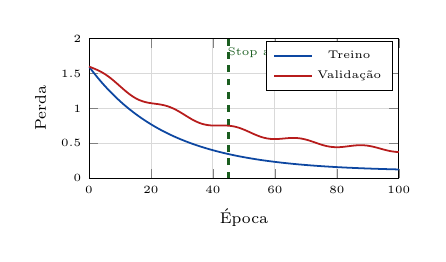
\begin{tikzpicture}[scale=0.80]
\begin{axis}[xlabel={Época},ylabel={Perda},
  width=6.5cm,height=3.8cm,
  xmin=0,xmax=100,ymin=0,ymax=2,
  grid=major,grid style={gray!30},
  tick label style={font=\tiny},
  label style={font=\scriptsize},
  legend style={font=\tiny}]
\addplot[deepblue,thick,domain=0:100,samples=100] 
  {1.5*exp(-0.04*x)+0.1};
\addlegendentry{Treino}
\addplot[deepred,thick,domain=0:100,samples=100]
  {1.3*exp(-0.025*x)+0.05*sin(deg(0.3*x))*exp(-0.005*x)+0.3};
\addlegendentry{Validação}
\draw[deepgreen,dashed,very thick] (axis cs:45,0)--(axis cs:45,2);
\node[font=\tiny,deepgreen] at (axis cs:55,1.8) {Stop aqui};
\end{axis}
\end{tikzpicture}
\begin{exampleblock}{}
\small
Early stopping é regularização implícita: equivale aproximadamente a $\ell_2$ com $\lambda \propto 1/t$.
\end{exampleblock}
\end{columns}
\end{frame}

%============================================================
\section{Introdução ao PyTorch}
%============================================================

\begin{frame}[fragile]{PyTorch — Conceitos Fundamentais}
\begin{columns}[T]
\column{0.50\textwidth}
\begin{block}{Tensores e Autograd}
\begin{lstlisting}
import torch
import torch.nn as nn

# Tensor com gradiente
x = torch.tensor([1.0, 2.0], 
                  requires_grad=True)
W = torch.randn(3, 2, 
                requires_grad=True)
b = torch.zeros(3, 
                requires_grad=True)

# Forward
z = W @ x + b
y = torch.relu(z)

# Backward (calcula gradientes)
loss = y.sum()
loss.backward()

# Gradientes disponiveis
print(W.grad)  # dL/dW
print(x.grad)  # dL/dx
\end{lstlisting}
\end{block}
\column{0.47\textwidth}
\begin{block}{Componentes Principais}
\small
\begin{tabular}{lp{3.5cm}}
\texttt{torch.Tensor} & Tensor N-dimensional com autograd \\
\texttt{nn.Module} & Classe base para camadas/modelos \\
\texttt{nn.Linear} & Camada totalmente conectada \\
\texttt{nn.ReLU/Sigmoid} & Ativações \\
\texttt{optim.SGD/Adam} & Otimizadores \\
\texttt{DataLoader} & Iterador sobre datasets \\
\texttt{loss.backward()} & Computa gradientes \\
\texttt{optim.step()} & Atualiza pesos \\
\end{tabular}
\end{block}
\begin{alertblock}{Dica: \texttt{.zero\_grad()}}
\small
PyTorch \textbf{acumula} gradientes. Sempre chame \texttt{optimizer.zero\_grad()} antes de \texttt{backward()}!
\end{alertblock}
\end{columns}
\end{frame}

%------------------------------------------------------------
\begin{frame}[fragile]{PyTorch — Loop de Treinamento Padrão}
\begin{lstlisting}
import torch, torch.nn as nn, torch.optim as optim
from torch.utils.data import DataLoader

# 1. Definir modelo
model = nn.Sequential(
    nn.Linear(784, 256), nn.ReLU(),
    nn.Linear(256, 128), nn.ReLU(),
    nn.Linear(128, 10)
)

# 2. Perda e otimizador
criterion = nn.CrossEntropyLoss()
optimizer = optim.Adam(model.parameters(), lr=1e-3)

# 3. Loop de treino
def train_epoch(model, loader, optimizer, criterion):
    model.train()
    total_loss = 0.0
    for X_batch, y_batch in loader:
        optimizer.zero_grad()           # Zera gradientes acumulados
        logits = model(X_batch)         # Forward pass
        loss = criterion(logits, y_batch)  # Calcula perda
        loss.backward()                 # Backpropagation
        optimizer.step()                # Atualiza pesos
        total_loss += loss.item()
    return total_loss / len(loader)
\end{lstlisting}
\end{frame}

%============================================================
\section{Implementação: MNIST com PyTorch}
%============================================================

\begin{frame}[fragile]{MNIST — Carregamento e Preparação dos Dados}
\begin{lstlisting}
import torch
import torch.nn as nn
import torch.optim as optim
from torchvision import datasets, transforms
from torch.utils.data import DataLoader

# Transformacoes: tensor + normalizacao (media=0.1307, std=0.3081)
transform = transforms.Compose([
    transforms.ToTensor(),
    transforms.Normalize((0.1307,), (0.3081,))
])

# Download automatico do MNIST
train_dataset = datasets.MNIST(root='./data', train=True,
                                download=True, transform=transform)
test_dataset  = datasets.MNIST(root='./data', train=False,
                                download=True, transform=transform)

train_loader = DataLoader(train_dataset, batch_size=64, 
                           shuffle=True,  num_workers=2)
test_loader  = DataLoader(test_dataset,  batch_size=1000,
                           shuffle=False, num_workers=2)

print(f"Treino: {len(train_dataset)} amostras")
print(f"Teste:  {len(test_dataset)} amostras")
print(f"Formato de uma imagem: {train_dataset[0][0].shape}")
# -> torch.Size([1, 28, 28])
\end{lstlisting}
\end{frame}

%------------------------------------------------------------
\begin{frame}[fragile]{MNIST — Arquitetura do MLP}
\begin{lstlisting}
class MLP_MNIST(nn.Module):
    """MLP para classificacao do MNIST.
    
    Arquitetura: 784 -> 512 -> 256 -> 128 -> 10
    Ativacao: ReLU nas camadas ocultas
    Regularizacao: Dropout(0.3)
    """
    def __init__(self, dropout_p: float = 0.3):
        super().__init__()
        self.flatten = nn.Flatten()          # [B,1,28,28] -> [B,784]
        self.network = nn.Sequential(
            nn.Linear(784, 512),
            nn.ReLU(),
            nn.Dropout(p=dropout_p),
            nn.Linear(512, 256),
            nn.ReLU(),
            nn.Dropout(p=dropout_p),
            nn.Linear(256, 128),
            nn.ReLU(),
            nn.Linear(128, 10)              # logits (sem softmax)
        )
        self._init_weights()
    
    def _init_weights(self):
        """Inicializacao de Kaiming para camadas ReLU."""
        for m in self.modules():
            if isinstance(m, nn.Linear):
                nn.init.kaiming_normal_(m.weight, nonlinearity='relu')
                nn.init.zeros_(m.bias)
    
    def forward(self, x: torch.Tensor) -> torch.Tensor:
        x = self.flatten(x)
        return self.network(x)
\end{lstlisting}
\end{frame}

%------------------------------------------------------------
\begin{frame}[fragile]{MNIST — Treinamento Completo}
\begin{lstlisting}
def evaluate(model, loader, criterion, device):
    model.eval()
    total_loss, correct = 0.0, 0
    with torch.no_grad():
        for X, y in loader:
            X, y = X.to(device), y.to(device)
            logits = model(X)
            total_loss += criterion(logits, y).item()
            correct += (logits.argmax(1) == y).sum().item()
    return total_loss/len(loader), correct/len(loader.dataset)

device = torch.device('cuda' if torch.cuda.is_available() else 'cpu')
model = MLP_MNIST(dropout_p=0.3).to(device)
criterion = nn.CrossEntropyLoss()
optimizer = optim.Adam(model.parameters(), lr=1e-3, weight_decay=1e-4)
scheduler = optim.lr_scheduler.StepLR(optimizer, step_size=5, gamma=0.5)

EPOCHS = 15
for epoch in range(1, EPOCHS + 1):
    model.train()
    train_loss = 0.0
    for X, y in train_loader:
        X, y = X.to(device), y.to(device)
        optimizer.zero_grad()
        loss = criterion(model(X), y)
        loss.backward()
        optimizer.step()
        train_loss += loss.item()
    scheduler.step()
    val_loss, val_acc = evaluate(model, test_loader, criterion, device)
    print(f"Ep {epoch:02d} | Loss Treino: {train_loss/len(train_loader):.4f}"
          f" | Loss Val: {val_loss:.4f} | Acc Val: {val_acc*100:.2f}%")
\end{lstlisting}
\end{frame}

%------------------------------------------------------------
\begin{frame}[fragile]{MNIST — Resultados e Visualização}
\begin{columns}[T]
\column{0.55\textwidth}
\begin{block}{Resultados Esperados}
\small
\begin{tabular}{lcc}
\toprule
Configuração & Acurácia Teste & Épocas \\
\midrule
MLP 784-512-256-128-10 & $\sim$98.2\% & 15 \\
+ Dropout(0.3) & $\sim$98.4\% & 15 \\
+ Weight Decay & $\sim$98.5\% & 15 \\
+ LR Scheduler & $\sim$98.6\% & 15 \\
\bottomrule
\end{tabular}
\end{block}
\begin{lstlisting}
# Visualizar predicoes
import matplotlib.pyplot as plt

model.eval()
X_sample, y_sample = next(iter(test_loader))
with torch.no_grad():
    preds = model(X_sample.to(device)
            ).argmax(1).cpu()

fig, axes = plt.subplots(2, 5, figsize=(10,4))
for ax, img, pred, true in zip(
        axes.flat, X_sample[:10], 
        preds[:10], y_sample[:10]):
    ax.imshow(img.squeeze(), cmap='gray')
    color = 'g' if pred==true else 'r'
    ax.set_title(f"Pred:{pred}", color=color)
    ax.axis('off')
plt.tight_layout()
plt.savefig('mnist_predictions.png')
\end{lstlisting}
\column{0.42\textwidth}
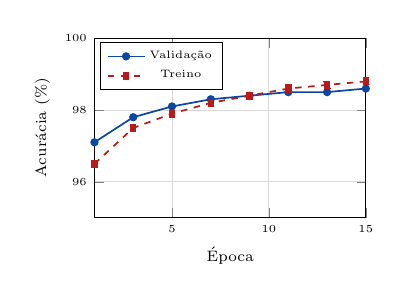
\begin{tikzpicture}[scale=0.78]
\begin{axis}[xlabel={Época},ylabel={Acurácia (\%)},
  width=6cm,height=4.5cm,
  xmin=1,xmax=15,ymin=95,ymax=100,
  grid=major,grid style={gray!30},
  tick label style={font=\tiny},
  label style={font=\scriptsize},
  legend style={font=\tiny,at={(0.02,0.98)},anchor=north west}]
\addplot[deepblue,thick,mark=*,mark size=1.5pt] 
  coordinates {(1,97.1)(3,97.8)(5,98.1)(7,98.3)
               (9,98.4)(11,98.5)(13,98.5)(15,98.6)};
\addlegendentry{Validação}
\addplot[deepred,thick,mark=square*,mark size=1.5pt,dashed]
  coordinates {(1,96.5)(3,97.5)(5,97.9)(7,98.2)
               (9,98.4)(11,98.6)(13,98.7)(15,98.8)};
\addlegendentry{Treino}
\end{axis}
\end{tikzpicture}
\begin{alertblock}{Referência MNIST}
\small
Estado da arte: $>99.7\%$ (CNN). MLPs atingem $\sim$98.5\% — suficiente para entender os fundamentos sem convolução.
\end{alertblock}
\end{columns}
\end{frame}

%============================================================
% Slide de Resumo e Referências
%============================================================

\begin{frame}{Resumo da Aula}
\begin{columns}[T]
\column{0.48\textwidth}
\begin{block}{Parte I — Teórico}
\small
\begin{itemize}
  \item[\checkmark] Contexto histórico: McCulloch-Pitts $\to$ Deep Learning
  \item[\checkmark] Formalismo: camadas, pesos, ativações
  \item[\checkmark] Cálculos manuais: forward pass
  \item[\checkmark] Funções de ativação: sigmoid, ReLU, softmax
  \item[\checkmark] XOR: prova de limitação + solução MLP
  \item[\checkmark] Design de arquiteturas
  \item[\checkmark] Loss functions: MSE, BCE, CCE, Huber, Focal
  \item[\checkmark] Backpropagation: história e matemática
  \item[\checkmark] Grafos computacionais
  \item[\checkmark] Regularização: $\ell_1$, $\ell_2$, Dropout, Early Stopping, Augmentation
\end{itemize}
\end{block}
\column{0.48\textwidth}
\begin{block}{Parte II — Prática}
\small
\begin{itemize}
  \item[\checkmark] PyTorch: tensores e autograd
  \item[\checkmark] \texttt{nn.Module}, \texttt{DataLoader}, loop de treino
  \item[\checkmark] Implementação MLP para MNIST ($\sim$98.5\%)
\end{itemize}
\end{block}
\begin{block}{Próximas Aulas}
\small
\begin{itemize}
  \item Redes Convolucionais (CNN)
  \item Otimização avançada (Adam, RMSProp, momentum)
  \item Batch Normalization
  \item Arquiteturas modernas (ResNet, Transformers)
\end{itemize}
\end{block}
\begin{alertblock}{Leitura Obrigatória}
\small
Goodfellow et al., Cap.\ 6 (\textit{Deep Feedforward Networks}) e Cap.\ 7 (\textit{Regularization}).
\end{alertblock}
\end{columns}
\end{frame}

%------------------------------------------------------------
\begin{frame}{Referências Bibliográficas}
\small
\begin{thebibliography}{9}
  \bibitem{goodfellow2016}
    I. Goodfellow, Y. Bengio, A. Courville.
    \textit{Deep Learning}. MIT Press, 2016.
    \href{https://www.deeplearningbook.org}{\texttt{deeplearningbook.org}}

  \bibitem{rumelhart1986}
    D. Rumelhart, G. Hinton, R. Williams.
    ``Learning representations by back-propagating errors.''
    \textit{Nature}, 323, 1986.

  \bibitem{minsky1969}
    M. Minsky, S. Papert.
    \textit{Perceptrons: An Introduction to Computational Geometry}.
    MIT Press, 1969.

  \bibitem{hornik1991}
    K. Hornik. ``Approximation capabilities of multilayer feedforward networks.''
    \textit{Neural Networks}, 4(2), 1991.

  \bibitem{srivastava2014}
    N. Srivastava et al. ``Dropout: A Simple Way to Prevent Neural Networks from Overfitting.''
    \textit{JMLR}, 15(1), 2014.

  \bibitem{nair2010}
    V. Nair, G. Hinton. ``Rectified Linear Units Improve Restricted Boltzmann Machines.''
    \textit{ICML}, 2010.
\end{thebibliography}
\end{frame}

%------------------------------------------------------------
\begin{frame}
  \centering
  \vspace{1.5cm}
  {\Huge\bfseries\color{deepblue} Obrigado!}\\[1.5cm]
  {\large Dúvidas?}\\[1cm]
  
\begin{tikzpicture}
    \draw[deepblue,line width=2pt] (0,0) -- (8,0);
  \end{tikzpicture}\\[0.8cm]
  {\small\color{gray}
  Baseado em: Goodfellow, Bengio \& Courville — \textit{Deep Learning} (MIT Press, 2016)\\
  Código disponível em: \texttt{github.com/\ldots/mlp-lecture}}
\end{frame}

\end{document}
